\documentclass[10pt]{article}

\addtolength{\oddsidemargin}{-.875in}
\addtolength{\evensidemargin}{-.875in}
\addtolength{\textwidth}{1.75in}

\addtolength{\topmargin}{-.875in}
\addtolength{\textheight}{1.75in}

\openup 1em

%macro for commenting
\usepackage{color}
\newcommand{\leo}[1]{{\color{blue}{\it leo: #1}}}

% \newcommand{\Xbeta}{ X_i \theta}
\newcommand{\xbeta}{ x_i \beta}
\newcommand{\xtheta}{ x_i \theta}
% \newcommand{\xbetaij}{ x_{ij}^T \theta}
\newcommand{\sgamma}{s_{ij}^T\gamma_i}

\usepackage[round]{natbib}

\usepackage{rotating}
\usepackage{graphicx}
\usepackage{subcaption}

\usepackage{float}
\usepackage{bbm}

\usepackage{amsthm,amsmath, amssymb} 
\usepackage{mathrsfs}
\usepackage{subcaption}
\usepackage{nicefrac}

\newtheorem{theorem}{Theorem}
\newtheorem{lemma}{Lemma}
\newtheorem{corollary}{Corollary}
\newtheorem{remark}{Remark}


\usepackage{algorithm}
\usepackage{algpseudocode}

%\usepackage{mhequ}
\newcommand{\be}{\begin{equation}\begin{aligned}}
\newcommand{\ee}{\end{aligned}\end{equation}}
\newcommand{\bb}[1]{\mathbb{#1}}
\newcommand{\mc}[1]{\mathcal{#1}}
\DeclareMathOperator{\Binom}{Binomial}
\DeclareMathOperator{\No}{No}
\DeclareMathOperator{\PG}{PG}
\DeclareMathOperator{\IG}{Inverse-Gamma}
\DeclareMathOperator{\Ga}{Gamma}
\DeclareMathOperator{\Bern}{Bernoulli}
\DeclareMathOperator{\U}{Uniform}
\DeclareMathOperator{\Poi}{Poisson}
\DeclareMathOperator{\NB}{NB}
\DeclareMathOperator{\cov}{cov}
\DeclareMathOperator{\var}{var}
\DeclareMathOperator{\diag}{diag}
\DeclareMathOperator{\Diag}{Diag}
\newcommand{\KL}[2]{\textnormal{KL}\left(#1 \parallel #2\right)}

\DeclareMathOperator{\1}{\mathbbm{1}}


\DeclareMathOperator{\bigO}{\mc O}



\thispagestyle{empty}
\baselineskip=28pt

\title{\textbf{Extrinsic Prior for Simple and Efficient\\ Bayesian Modeling with Parameter Constraints}}
\author{Leo Duan, Akihiko Nishimura, David Dunson}
\date{}
\begin{document}

\maketitle


{\bf Abstract:} Parameter constraints are commonly seen in statistical models, such as linear inequality, simplex constraint, parameter ordering, monotonicity, orthogonality, etc. Bayesian approach is useful for uncertainty quantification in constrained space. Although customized solutions have been developed in the past, it is still difficult to carry out estimation in general cases, especially when posteriors lack closed-form. In this paper, we propose a simple and general solution by replacing constraints with strongly informative prior. Through this {\it extrinsic} prior, the parameter support is relaxed to a less restrictive space, where conventional tools such as Hamiltonian Monte Carlo can be exploited to obtain approximate posterior efficiently. If one needs to uphold the constraints, the posterior sample can be projected back to the constrained space to obtain exact solution. We illustrate various cases with equality and inequality constraints. As priors are no longer limited to ones with closed-form posterior, more distribution families can be chosen for the constrained parameters; constraints can be freely adopted for desired property, such as improving convergence. Theory is developed and novel statistical applications under constraints are demonstrated.
\vskip 12pt

%\baselineskip=12pt
%\par\vfill\noindent
{\noindent  KEY WORDS:  Constraint relaxation; Euclidean Embedding; Monotone Dirichlet;  Soft Constraint; Stiefel Manifold; Projected Markov chain}
%\par\medskip\noindent
%\clearpage\pagebreak\newpage
\pagenumbering{arabic}

\section{Introduction}

Constraints are common in modern statistical models. For example, functional data anaylsis often imposes constraint on shape, such as monotonicity or convexity on curves \citep{kelly1990monotone}; matrix and tensor decomposition utilize orthonormality to remove scaling and rotation that impacts identifiability \citep{uschmajew2010well}; many manifolds such as simplex can be considered as sub-manifolds of a Euclidean space via some constraint.

%\leo{I'll move this paragraph to discussion}
%When data are in constrained space, parameters can enter the likelihood via an integral without closed-form, leading to ``doubly intractable'' problem. Various successful solutions have been proposed for this issue \citep{murray2012mcmc,rao2016data}. 

When parameters are constrained, challenges often arise in their estimation. Optimization literature often relies on Lagrange and Karush-Kuhn-Tucker multipliers for point estimate under equality and inequality constraints \citep{boyd2004convex}. However, uncertainty quantification is difficult via optimization, as asymptotic result for variance estimation in Euclidean space no longer holds in constrained space. In this regard, Bayesian approach is particularly advantageous.

There have been a variety of customized solutions developed for specific constraints. One popular strategy rely on picking constrained prior with posterior easy to sample. For example, for modeling othornormal matrices on the Stiefel manifold, Bingham-von-Mises-Fisher distribution \citep{khatri1977mises,hoff2009simulation} is a parametric family with  posterior conjugacy, which gives its popularity in matrix and tensor decomposition. To improve its flexibility, \cite{lin2016bayesstiefel} extends the matrix von-Mises-Fisher distribution via non-parametric Bayes approach. When the simple posterior form is not directly available, another strategy is to bypass the constraint via re-parameterization. The famous example is the stick-breaking construction for Dirichlet distribution and process. The re-parameterization essentially utilizes the coordinate system of the simplex, and circumvents the norm constraint on the probability vertices. Both strategies ``intrinsically'' meet the constraint, therefore are commonly referred as intrinsic approaches. Despite their success, there are several issues. When the parameter is multi-dimensional, one often has to use Gibbs sampling to update one dimension at a time, leading to inefficient computation. Moreover, the closed-form of posterior distribution is prone to break under slightly more advanced model or complicated data assumption. For example, for modeling population of undirected networks, symmetry in each network can disrupt the posterior conjugacy in orthogonal tensor decomposition, demanding new customized sampling algorithm to be developed. As another example, additional structure (such as ordering) on the probability simplex breaks the stick-breaking formulation.

These drawbacks have motivated the development of extrinsic approaches. The key idea is to first generate proposal freely in a conventional space (such as Euclidean space), then transform it back to the constrained space. One early work can be traced back to \cite{gelfand1992bayesian}, who suggested Gibbs sampling to first generate proposal in unrestricted region, then only accepting those falling inside the constraint space. One critical issue is that unrestricted proposal can have significant mass outside the constraint region, resulting in a high rejection rate. Replacing rejection sampling, \cite{lin2014monogp} and \cite{lin2016extrinsic} utilize a deterministic projection to map the unconstrained posterior into the constrained space and obtain monotonicity and manifold-valued regression. In Hamiltonian Monte Carlo, \cite{neal2011mcmc} suggested using large penalty to create an energy wall to induce simple space truncation, and accept proposal only when it is inside the truncated space. \cite{pakman2014exact} applied similar idea in making the generation of truncated multivariate normal more efficient. These cases work well, but those settings are very specific and there is a clear lack of general and simple approach. 

In this paper, we propose a new extrinsic approach, by parameterizing constraints as a limiting case of strongly informative prior. We refer them as extrisic priors. We then relax the effective support of the prior to a neighborhood of constraint space, obtaining posterior via efficient tools such as conventional Hamiltonian Monte Carlo (HMC). When the constraints need to upheld strictly, the approximation can be corrected with a simple projection, followed by a Metropolis-Hastings step with high acceptance probability. Compared to other manifold based methods such as Riemannian and geodesic HMC \citep{girolami2011riemann,byrne2013geodesic}, our approach is efficient in computation and simple to implement via highly automatic software like STAN. The simplicity enables a larger spectrum of prior to be chosen and more free adoption of constraints in modeling. Theoretic studies are conducted and original models are shown in simulations and data application.

\section{Method}

We consider parameters $\theta$ in a constrained space $\mc D$. Both $\theta$ and $\mc D$ can be high or infinite-dimensional. Letting $\mc D$  be equipped with a $\sigma$-field $\mathscr D$, the standard Bayesian approach assigns a prior for $\theta$ in $\mc D$, based on a density $\pi_{0,\mc D}(\theta)$ in a separable space $(\mc D, \mathscr D)$. In intrinsic approaches, priors are chosen for computational conveniences so that the posterior can be easily sampled strictly inside $\mc D$. Clearly, the available choices in both priors and constraints are very limited.

Instead, we consider extrinsic approaches by estimating $\theta$ in a larger space $\mc R$ where $\mc D\in \mc R$. We first provide a probabilistic justification. Assuming $\pi_{0,\mc D}(\theta)$ is proper $\int_{\mc D} \pi_{0,\mc D}(\theta) d\theta <\infty$, then the constrained prior can be viewed as a conditional density, based on another density $\pi_{0,\mc R}(\theta)$ in $(\mc R, \mathscr R)$ with $\mathscr R$ as the $\sigma$-field of $\mc R$:

\begin{equation}
\begin{aligned}
\pi_{0,\mc D}(\theta)= \pi_{0,\mc R}(\theta \mid \theta \in \mc D) = \frac{ \pi_{0,\mc R}(\theta) \mathbbm{1}_{\theta\in \mc D} }{ \int_{\mc D}  \pi_{0,\mc R}(\theta)d\theta }.
\end{aligned}
\end{equation}
where $\mathbbm{1}_{\theta \in \mc D}=1$ when $\theta \in \mc D$, $0$ otherwise. For example, in matrix von Mises--Fisher distribution for $\theta$ on Stiefel manifold $\mc D(\theta)=\mc V(N,d)$, $\pi_{0,\mc D}=\frac{\exp(\text{tr}(F'\theta))\mathbbm{1}_{\theta'\theta=I_d}}{_0G_1(F)}$, with $_0G_1(F)= \int_{\mc D} \exp(\text{tr}(F'\theta)) d\theta$ as confluent hypergeometric limit function. Letting $L(\theta;y)$ be the likelihood function and $y$ be the observed data, the posterior can be obtained via:

\begin{equation}
\begin{aligned}
\label{exact_posterior}
\pi(\theta \mid y, \theta \in \mc D) = \frac{ L(\theta;y)\pi_{0,\mc D}(\theta)}{\int_{\mc D} L(\theta;y)\pi_{0,\mc D}(\theta) d\theta } = \frac{ L(\theta;y)\pi_{0,\mc R}(\theta) \mathbbm{1}_{\theta\in \mc D} }{\int_{\mc D} L(\theta;y)\pi_{0,\mc R}(\theta) d\theta },
\end{aligned}
\end{equation}
where the last equality holds because $\int_{\mc D}  \pi_{0,\mc R}(\theta) d\theta$ is a finite constant. Therefore, \eqref{exact_posterior} shows that if $\pi_{0,\mc R}(\theta) \mathbbm{1}_{\theta\in \mc D}$ is proper,
one can use any prior in $\mc R$ to couple with constraint, and obtain valid posterior in $\mc D$,


\subsection{Extrinsic Prior}

One obvious extrinsic approach utilizing \eqref{exact_posterior} is to first generate proposal in $\mc R$ based on $L(\theta;y)\pi_{0,\mc R}(\theta)$ (assuming it is proper), then accepting it when it falls in $\mc D$ \citep{gelfand1992bayesian}. However, when the ratio of probabilities $Pr(\theta\in \mc D \mid y) / Pr(\theta\in \mc R \mid y) \approx 0$, commonly in equality constraint, this would lead to most of the proposals being rejected.

We propose a different strategy. Instead of ignoring $\mathbbm{1}_{\theta\in \mc D} $ in the first step, we approximate it with a strongly informative prior with density $\mc K(\theta)$. This prior has support $\mc S$ that $\mc D\subset\mc S\subset\mc R$ with its mass concentrated around $\mc D$. Then one can first obtain posterior based on density proportional to $L(\theta;y)\pi_{0,\mc R}(\theta)\mc K(\theta)$.

In this paper, we focus on $\mc D$ that can be embedded in $\mc R$ via equality and inequality constraints, although other types of constraints can be incorporated similarly. Letting there be $m$ equalities and $l$ inequalities, this leads to embedding $\mc D = \{ \theta \in \mc R: E_k(\theta)=0 \text{ for } k=1,\ldots,m, \quad G_{k'}(\theta)\le 0  \text{ for } k'=1,\ldots,l \}$, where $E_k(.)$ and $G_{k'}(.)$ are functions that map from $\mc R$ to real line $\mathbb R$. Then the indicator function in \eqref{exact_posterior} can be broken into $\mathbbm{1}_{\theta\in \mc D} = \prod_k \mathbbm{1}_{E_k(\theta)=0} \cdot \prod_{k'}\mathbbm{1}_{G_k'(\theta)\le 0}$.


We now form extrinsic prior $\mc K(\theta)$ by replacing each indicator functions with a kernel function $K_.(.)$, this yields posterior:

\begin{equation}
\begin{aligned}
\label{extrinsic_prior}
\pi_{\mc K}(\theta \mid y) & \propto L(\theta;y)\pi_{0,\mc R}(\theta) \mc K(\theta) \\
&= L(\theta;y)\pi_{0,\mc R}(\theta) \cdot \prod_{k=1}^{m} K_{1,k}\Big( | E_k(\theta)| \Big) \cdot \prod_{k'=1}^{l} K_{2,k'}\Big( \big( G_{k'}(\theta) \big)_+ \Big)
\end{aligned}
\end{equation}
where $(x)_+ = x$ if $x>0$, $0$ if $x\le 0$. For example, one simple kernel is the truncated Gaussian kernel $K_{i,k}(x) = \exp( -{\lambda_{i,k} x^2}) \mathbbm{1}_{x<\varepsilon(\lambda_{i,k})}$, where $\varepsilon(\lambda_{i,k})$ is a truncation bound depends on $\lambda_{i,k}$ (more will be explained in next section). Generally, the posterior value of functions $|E_k(\theta)|\in [0,\infty)$ or $(G_{k'}(\theta))_+ \in [0,\infty)$ represent the amount of relaxation for each constraint, where $0$ represents no relaxation. Each kernel $K_{i,k}$ satisfies $K_{i,k}(0)=1$ when the constraints are met; the tolerable amount of relaxation is controlled by hyper-parameter $\lambda_{i,k}$. When $\lambda_{i,k} \rightarrow \infty$, the kernel becomes a point mass at $0$. Therefore, \eqref{exact_posterior} is a special limiting case of \eqref{extrinsic_prior}.

When $\lambda_{i,k}$'s take large but finite values, they give rise to a continuous relaxation of the sharp boundary of the indicator function. The relaxation allows the posterior $\theta$ to be easily sampled in $\mc R$ under the influence of the strongly informative prior $\mc K(\theta)$. At the same time, since posteriors are generated in a tight neighborhood of $\mc D$, they can be easily projected back to $\mc D$ as to produce exact posterior in $\mc D$, if needed. We use subscript $\mc K$ to denote posterior $\pi_{\mc K}(\theta \mid y)$, which can be viewed as an approximation to $\pi(\theta \mid y)$ in \eqref{exact_posterior}. We will now refer $\pi_{\mc K}(\theta \mid y)$ as ``extrinsic posterior''.

\subsection{Control of Constraint Relaxation}

We first obtain a control of constraint relaxation, in terms of the posterior values of $|E_k(\theta)|$ and $(G_{k'}(\theta))_+$. Letting $v$ represents their values, the control can be achieved via a bounded prior support near $0$ for each kernel $\int_{v<\varepsilon} \mc C_{i,k}(v)  dv= 1$, with  $\mc C_{i,k}(v) = K_{i,k}(v) / \int_{\mc R}K_{i,k}(v) dv$. The pre-specified constant $\varepsilon$ represents the element-wise tolerance for violating each constraint. The bounded prior support allows us to theoretically control the posterior approximation error. With $\mc K(\theta) \propto \prod_{i,k} \mc C_{i,k}(x)$ is the joint extrinsic prior density, since $\pi_{\mc K}(\theta \mid y) \ll \mc K(\theta)$, the posterior for each constraint relaxation is bounded in $[0,\varepsilon)$ with probability $1$.

In practice, one may wish to utilize a kernel $K^*_{i,k}(x)$, orginally with unbounded support on $[0,\infty)$ for computing conveniences. To adapt them for bounded support in the relaxation $v$, one can first choose $\lambda_{i,k}$ to have $\int_{v<\varepsilon} \mc K^*_{i,k}(x)/ \big( \int_{\mc R} K^*_{.}(v) dv\big ) = 1-\eta$ with $\eta$ small, then apply truncation $K_{i,k}(v)= K^*_{i,k}(v) \mathbbm{1}_{v<\varepsilon}$ to induce $v<\varepsilon$ almost surely. In most cases, the truncation is only nominal for a theoretic guarantee; in computation it is rarely used. For example, in Gaussian kernel $\exp( -{\lambda x^2})$ assigns $x<4/\sqrt{2\lambda}$ with probability $0.99993$ apriori; for posterior sampling, one can first do an untruncated sampling, then reject those $x>\varepsilon=4/\sqrt{2\lambda}$, which is quite rare due to the small prior probability. 

To illustrate the control of constraint relaxation, we assume a simple scenario of generating posterior from a truncated Gaussian distribution $\theta \mid y \sim \No_{(\alpha,\beta)}(0,1)$, with mean $0$ and variance $1$ and truncation $\theta\in (\alpha,\beta)$. The exact and extrinsic posterior densities are:

$$\pi(\theta\mid y)\propto \exp(-\frac{\theta^2}{2}) \mathbbm{1}_{\theta\in(\alpha,\beta)}, \quad \pi_{\mc K}(\theta\mid y)\propto \exp(-\frac{\theta^2}{2}) K \left ( (\alpha - \theta)_+ \right) K \left ( ( \theta - \beta)_+ \right).$$
with $K(x)= \exp( - \lambda x^2)\mathbbm{1}_{x<4/\sqrt{2\lambda}}$. We set $(\alpha, \beta)=(1,2)$. Figure~\ref{truncated_normal} plots the unnormalized densities under the exact and extrinsic posteriors with different $\lambda$'s. The extrinsic posterior densities inside $\mc D = (1,2)$ are the same as the exact one, up to a constant difference due to normalization. Outside $\mc D$, the larger $\lambda$ leads to more rapid decline of density and therefore smaller constraint relaxation $(\alpha - \theta)_+ $ and $ ( \theta - \beta)_+$.

\begin{figure}[H]
 \centering
 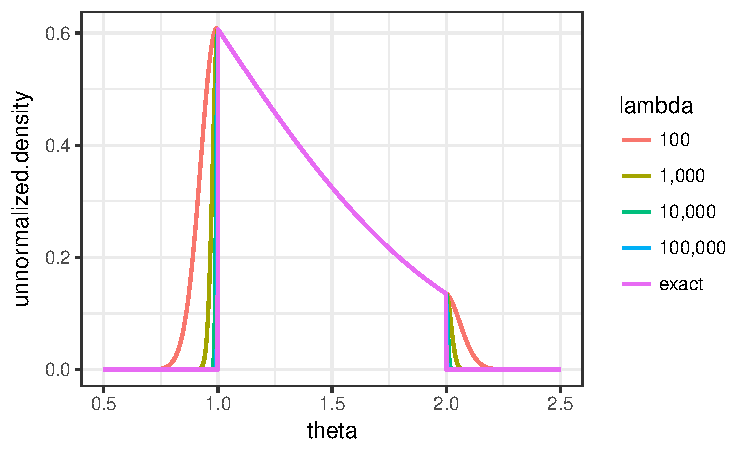
\includegraphics[width=0.5\textwidth]{density_truncated_normal}
\caption{Unnormalized densities for truncated normal $\No_{(1,2)}(0,1)$, under exact $\pi(\theta\mid y)$ and extrinsic posterior $\pi_{\mc K}(\theta\mid y)$. The exact density abruptly drops to $0$ on the two boundaries, while the approximating ones drop continuously. In the approximation, larger $\lambda$ is associated with lower tolerance for constraint relaxation ($( 1-\theta )_+$ and $( \theta - 2)_+$). All densities inside $(1,2)$ are the same up to a constant difference.}
\label{truncated_normal}
\end{figure}

It is temping to always induce almost $0$ relaxation with very large $\lambda$, however, in heavily constrained models such as the ones with equality constraint, the narrow distribution width in $\mc R$ will cause a adverse effect in some popular algorithms such as Hamiltonian Monte Carlo. In those cases, it is rather useful to have a slightly larger relaxation, then use projection to correct the imperfection. We will illustrate this in the next section.

\subsection{Hamiltonian Monte Carlo for Extrinsic Posterior Sampling}

Extrinsic posterior has support on a less restrictive space $\mc R$, where conventional sampling approach such as slice sampling, adaptive Metropolis-Hastings and Hamiltonian Monte Carlo (HMC) can be adopted easily. In this paper, we focus on estimation via HMC for its high-level automation aided by software and often good performance due to various adaptive algorithms \citep{hoffman2014no}. To be clear, this is different from Riemannian HMC that requires specific accommodation and heavy computation. The algorithm we use is simply conventional HMC in Euclidean space. In this section, we study the effects of choosing $\lambda$ on efficiency of Hamiltonian dynamics.

We assume $\theta$ is $d$-dimensional, $\mc R$ is a full or truncated Euchledean space in $\mathbb R^d$, and the constraint functions $E_k(\theta)$'s and $G_k(\theta)$'s  are differentiable with respect to $\theta$. We focus on the case where $\theta$ is continuous, although discrete extension is possible \citep{zhang2012continuous}. HMC augments a latent variable named ``veolicty'' or ``momentum'' $p\in \mathbb R^d$, the negative log-posterior function based on \eqref{extrinsic_prior} is

\begin{equation}
\begin{aligned}
H(\theta, p)& = U(\theta)+M(p),\\
\text{where } & U(\theta) = -\log\left\{ L(\theta;y)\pi_{0,\mc R}(\theta) \mc{E}(\theta) \right\},\\
& M(p) = \frac{p'\Sigma^{-1} p}{2},\end{aligned}
\end{equation}
with $\Sigma^{-1}$ a pre-specified positive definite matrix. Instead of taking random walk or Gibbs updating, HMC then update $\theta$ and $p$ via Hamiltonian dynamics, satisfying differential equations:

\begin{equation}
\begin{aligned}
\label{hamiltonian}
\frac{\partial \theta (t)}{\partial t} & =\frac{\partial H(\theta, p)}{\partial p} = \Sigma^{-1}p,\\
\frac{\partial p(t)}{\partial t}& =-\frac{\partial H(\theta, p)}{\partial \theta} = -\frac{\partial U(\theta)}{\partial \theta}.
\end{aligned}
\end{equation}

At the start of each iteration, the current state of $\theta$ is viewed as $\theta(0)$ and $p(0)$ randomly generated from $\No(0, \Sigma)$. The solution to \eqref{hamiltonian} yields $\theta(t)$ and $-p(t)$ as the new state. Since Hamiltonian system is symplectic, the negative log-posterior function is unchanged $H(\theta(t),p(t))=H(\theta(0),p(0))$. However, in most cases, \eqref{hamiltonian} lacks closed-form solution, one has to use discrete approximation, commonly leap-frog algorithm \citep{neal2011mcmc}:


\begin{equation}
\begin{aligned}
\label{leap-frog}
p(T+ \varepsilon/2) & = p(T) - \varepsilon/2 \frac{\partial U}{\partial  \theta } ( \theta (T)),\\
 \theta (T + \varepsilon) & =  \theta (T) + \varepsilon \Sigma^{-1}p(T+  \varepsilon/2),\\
p(T+ \varepsilon) &= p(T+ \varepsilon/2) - \varepsilon/2 \frac{\partial U}{\partial  \theta } ( \theta (T + \varepsilon)),
\end{aligned}
\end{equation}
for $T=0,\varepsilon, 2\varepsilon,\ldots, (L-1)\varepsilon$, with $\varepsilon$ known as the time step, and $L$ as the total leap-frog steps within one iteration. The sequence of $\{(p(T),\theta(T))\}_T$ form a trajectory of length $L+1$ in the space of $\mathbb R^{2d}$. Since this approximating update is deterministic and reversible, an Metropolis-Hastings (M-H) step can be taken at the end to accept $\theta(t)$ and $p(t)$ with probability 
$$1\wedge \exp  \left( - H(\theta(t),-p(t)) + H(\theta(0),p(0))\right)$$
 with $t=L\varepsilon$.
 
 
Since extrinsic prior replaces the constraint indicator $\mathbbm{1}_{\theta \in \mc D}$ with a continuous function, conventional HMC can be directly run in space $\mc R$. In HMC, finding optimal time step $\varepsilon$ is important. There exists a stability bound for $\epsilon$. When $\varepsilon$ is larger than this bound, $H$ diverges and grows exponentially with $L$, leading to very low acceptance rate in M-H step. When $\varepsilon$ is too small, each time step can only generate local update hence low computing efficiency. 
%For simple system such as $U(\theta)= {\theta^2}/{2\sigma^2}$, one can write \eqref{leap-frog} as a linear transfromation of $[\theta(T+\varepsilon),p(T+\varepsilon)]' = Q [ \theta(T),p(T)]'$ ($Q$ is a $2d\times 2d$ transition matrix), bounding the eigenvalues in $Q$ below magnitude $1$ determines the stability bound. 
Since most systems involve nonlinear transition, analytical bound is not available, but one can empirically optimize $\varepsilon$ to be close to this bound. This can be achieved via tuning for acceptance rate in the Metropolis-Hastings step. Specifically, given fixed $L$, one tunes $\varepsilon$ so that the acceptance rate is close to but slightly below $1$. Despite the technicality, the tuning of $\varepsilon$ is implemented in the mature HMC software such as STAN. We instead focus on how $\lambda$ can affect the stability bound itself.

For multiple-dimensional $\theta$ with $\Sigma=I$, the stability bound is roughly determined by the width of distribution in the most constrained direction  \citep{neal2011mcmc}. To provide an intuition, we focus on one  time step update $L=1$. Each update in leap-frog algorithm corresponds to $\theta(\varepsilon)=\theta(0) + \varepsilon  p(0) - \varepsilon^2/2  \frac{\partial U}{\partial  \theta } ( \theta (0)) = \theta(0) + \varepsilon  p(0) + O(\varepsilon^2)$. When the support in extrinsic posterior is narrow along certain direction, an move in $\varepsilon  p(0)$ can end in region with posterior density $0$ (associated with infinite $U(\theta(t))$). This is because we do not constrain $p(0)$, so that it is randomly generated in all direction of $\mathbb R^d$. On the other hand, a stable trajectory should approximately preserve $U(\theta(\varepsilon))+M(p(\varepsilon)) = U(\theta(0))+M(p(0))$, since $M(p)= p'p/2 \ge 0$, $U(\theta(\varepsilon))\le  U(\theta(0))+M(p(0))$. With initial velocity $p(0)\sim N(0, I)$ and finite $U(\theta(0))$, a stable trajectory should never move to region outside of support. Therefore, the stability bound on $\varepsilon$ is indeed impacted by the smallest width of posterior support.

Therefore in extrinsic prior, it is important to avoid creating a support too narrow. This could be possible with strong constraints like equality. When embedded in larger space, the approximate hyper-plane specified by equality extrinsic prior has its narrowest width as the amount of relaxation from strict equality. In such cases, very large $\lambda$ would force small stability bound on $\varepsilon$, creating computing bottleneck; instead, it is more efficient to use smaller $\lambda$ to induce more relaxation. On the other hand, inequality constraints often do not have this issue, as long as these inequalities do not induce narrow support. Therefore, one can often use large $\lambda$ in inequality extrinsic prior.

To illustrate, we consider generating posterior $\theta=(x_1,x_2)$ on a unit circle using von Mises--Fisher distribution, $\pi(\theta \mid y) \propto \exp(F'\theta)$ with $\theta'\theta =1$. This is a simple example of a random variable constraint on a $(2,1)$-Stiefel manifold $\mc D =\mc V(2,1)$. We set $F=(1,1)$ to induce a distribution widely spreaded over the manifold, generating great amount of uncertainty for assessing the sampling efficiency. We use extrinsic prior proportional to $K(\theta)= \exp(-\lambda (\theta'\theta -1)^2) \mathbbm{1}_{|\theta'\theta -1|<0.1}$. Geometrically, this prior expands the posterior support from a circle to a ring, with its width $|\theta'\theta -1|$ affected by $\lambda$.

\begin{figure}[H]
 \centering
    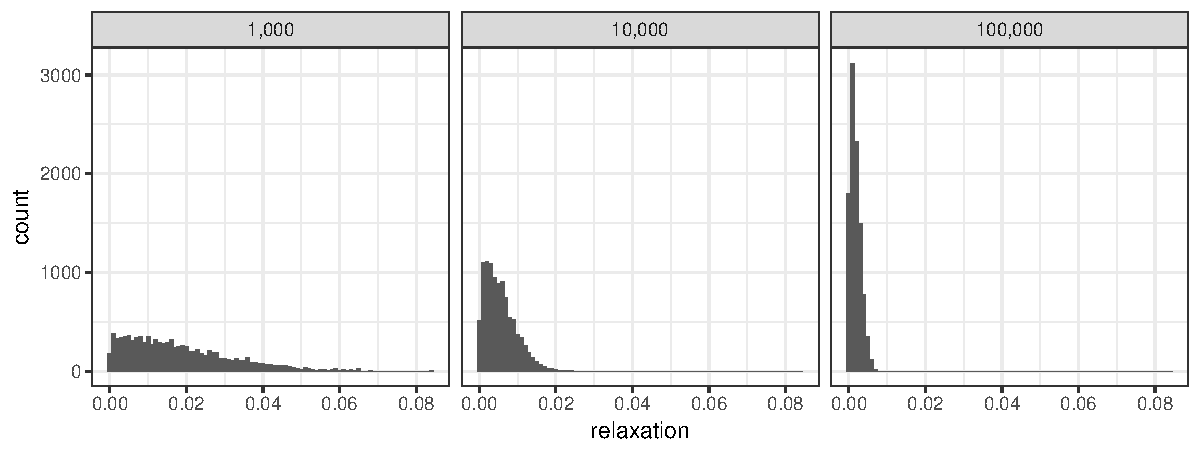
\includegraphics[width=0.8\textwidth]{unit_circle_violation}
  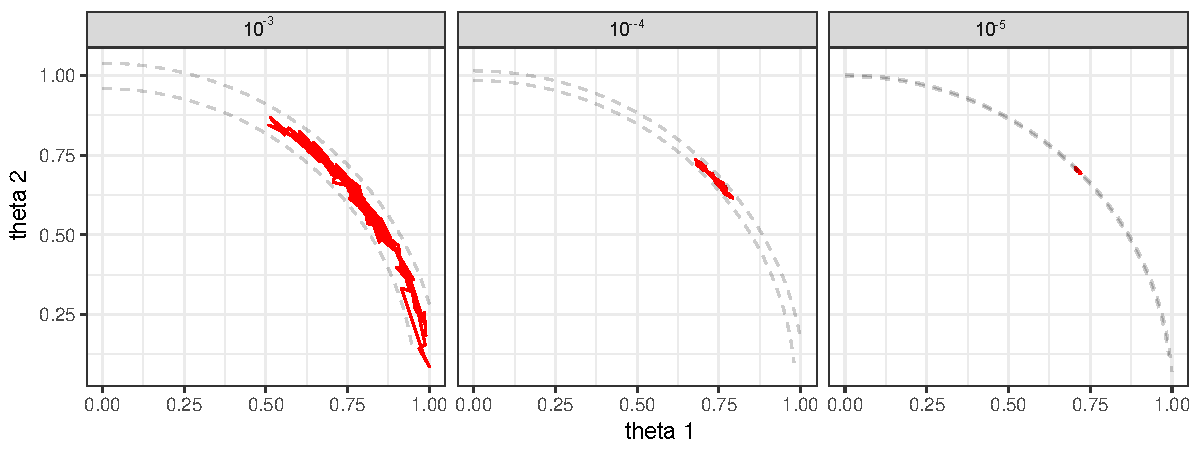
\includegraphics[width=0.8\textwidth]{unit_circle_100steps}
 % 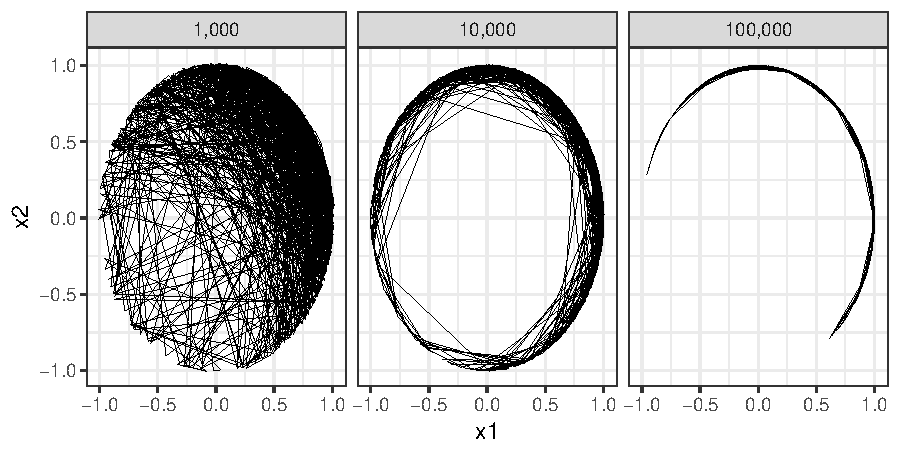
\includegraphics[width=0.8\textwidth]{unit_circle_path}
 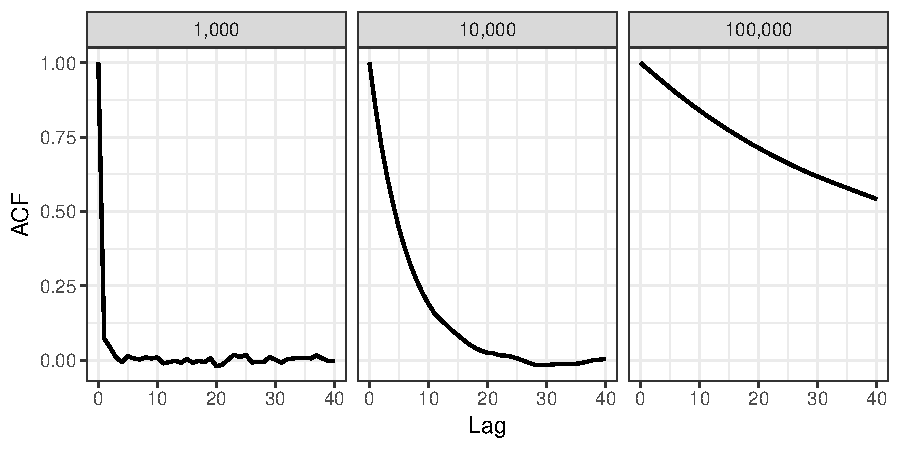
\includegraphics[width=0.8\textwidth]{unit_circle_acf}
\caption{Sampling posterior from a von Mises--Fisher distribution on a unit circle, using HMC with extrinc prior under $\lambda=10^3,10^4,10^5$. Row $1$ shows the posterior distribution of the constraint relaxation $|\theta'\theta -1|$; Row $2$ shows the path of $100$ leap-frog steps; Row $3$ shows the autocorrelation plot (ACF). Large $\lambda$ gives very small constraint relaxation, but suffers from slow mixing due to inefficient local update; smaller $\lambda$ increases the relaxation but results in excellent mixing.}
\label{unit_circle}
\end{figure}


We tested three different values of $\lambda = 10^3,10^4,10^5$. For each $\lambda$, we ran HMC for $10,000$ iterations, with $L=100$ leap-frog steps in each iteration. 
We set $\Sigma= \diag(1,1)$ in generating velocity $p$. During the initial $2,000$ iterations, the leap-frog step size $\varepsilon$ is tuned for an acceptance rate close to $0.8$, then it is fixed during the remaining part of Markov chain. The last $5,000$ iterations are used as posterior samples. Figure~\ref{unit_circle} plots the posterior distribution of constraint relaxation $|\theta'\theta -1|$, the sampling path and the autocorrelation function (ACF) for each Markov chain. Very large $\lambda=10^5$ has much less constraint relaxation; however, due to the small ring width, the Hamiltonian dynamics has to use small $\varepsilon$ and can only explore local space for each $100$ time steps. This results in a very slow mixing (large autocorrelation even at 40 lags). On the other hand, smaller $\lambda=10^3$ has slightly larger constraint relaxation, but allows much more efficient exploration of the space and excellent mixing performance. In general, we find that $\lambda=10^3$ is a good empirical value for all the equality constraints used in this paper.

\subsection{Soft and Hard Constraints}

We now introduce two new notions ``soft'' and ``hard'' constraints. Often, some model constraints are included as an extra means to improve convergence and identifiability. For example, the ordering of parameters are often used to address multi-modality under parameter permutation. In such cases, one can allow those constraints to be slightly relaxed without obviously impacting these objectives. We refer such relaxed constraint as soft constraint; in our framework, the extrinsic prior generates a soft constraint. One obvious benefit of soft constraint is that one can directly replaces the inconvenient model constraint by soft constraint, and use extrinsic posterior for statistical inference. Another benefit is to introduce some uncertainty on some constraint, and  allow the posterior to mildly violate these constraint if the data strongly suggests so.

%\leo{I hide this paragraph, because I want to use order constraint on simplex instead of on component means in the next example section}
% Moreover, another important advantage is that soft constraint can allow multiple conflicting constraints to co-exist in the same model. One example is the ordering of multivariate parameters $\theta_{i}=\{ \theta_{i1}, \theta_{i2},\ldots, \theta_{ip}\}$ over index $i=1,\ldots, n$. One can use kernel $\prod_{j=1}^p \prod_{i=1}^{n-1} K_j( (\theta_{i,j} - \theta_{i+1,j})_+)$ as an extrinsic prior to induce favoring of some ordering in all of the $p$ sub-dimensions. Then one could use $\lambda_j$ decreasing in $j$, to induces lower penality of order violation as $j$ increases.

On the other hand, there are some constraints that need to be upheld strictly, such the constraints embedding manifold in Euclidean space. We refer those as hard constraints. In the last example, the $2$-norm constraint needs to be always met in order to have parameter on the unit circle. Under this scenario, the extrinsic posterior is an approximation to posterior under hard constraint, hence needs to be corrected to have valid inference. We now describe a simple procedure in the next section.

\subsection{Correcting Projection for Hard Constraint}
 
 The extrinsic posterior $\pi_{\mc K}(\theta \mid y)$ is an approximation to \eqref{exact_posterior} under hard constraint. We now introduce a step to correct the approximation error, by projecting $\theta$ back to constrained space $\mc D$.
 
The Markov chain produced by HMC is geometrically ergodic under very general conditions \citep{livingstone2016geometric}. Letting $\theta^*$ be a random sample collected based on $\pi_{\mc K}(\theta \mid y)$, there exists deterministic projection $P: \mc R\rightarrow \mc D$ and obtain $\theta^*_{\mc D}= P(\theta^*)$. Using this as proposal machineary, one can construct another Markov chain with $\pi(\theta_{\mc D}  \mid y)$ as the target distribution. Letting the current state be $\theta_{\mc D} = P(\theta)$, we generate proposal $\theta^*_{\mc D}= P(\theta^*)$ and accept it with probability:

\begin{equation}
 \begin{aligned}
 1 \wedge \frac{\pi(\theta^*_{\mc D} \mid y) \pi_{\mc K}(\theta  \mid y) }{\pi(\theta_{\mc D}  \mid y)\pi_{\mc K}(\theta^* \mid y)} =  1 \wedge \frac{\ L(\theta^*_{\mc D};y)\pi_{0,\mc R}(\theta^*_{\mc D})  \cdot    L(\theta;y)\pi_{0,\mc R}(\theta)   \mc K(\theta)}{\ L(\theta_{\mc D};y)\pi_{0,\mc R}(\theta_{\mc D})   \cdot L(\theta^*;y)\pi_{0,\mc R}(\theta^*)   \mc K(\theta^{*})}.
 \end{aligned}
 \end{equation}
 
 This procedure converts a set of extrinsic posterior samples into a Markov chain with exact constrained posterior as the target. Simple projection often exists for common constraints and yields high acceptance rate. Because the extrinsic prior allows only very small relaxation of hard constraints, the projection gives very little change from $\theta$ to $\theta^*_D$. In the last example of unit circle, one can project by simply normalizing each $P(\theta^*) = \theta^*/||\theta^{*}||_2$. Since in the extrinsic posterior $||\theta^{*}||_2$ is very close to 1, the change is very small. We obtained the exact chain with acceptance rate of $0.98$.
 
 %skip this complicated projection for now, as it's mostly unnecessary
%The remaining task is then to optimize the projection with respect to the acceptance rate. Noting 

%\begin{equation}
%\begin{aligned}
%|\log( \frac{\pi(\theta^*_{\mc D} \mid y) \pi_{\mc K}(\theta  \mid y) }{\pi(\theta_{\mc D}  \mid y)\pi_{\mc K}(\theta^* \mid y)}) | \le |\log \left( \pi(\theta^*_{\mc D} \mid y) \right) - \log \left( \pi_{\mc K}(\theta^* \mid y) \right)| + |\log \left( \pi(\theta_{\mc D} \mid y)\right) - \log\left( \pi_{\mc K}(\theta \mid y)\right)|,
%\end{aligned}
%\end{equation}
%it is sensible choose $\theta_{\mc D}\in \mc D$ to minimize the difference $Q(\theta_{\mc D})=\left|\log( \pi(\theta_{\mc D} \mid y)) - \log( \pi_{\mc K}(\theta \mid y))\right|$ towards $0$ for each sample in the extrinsic posterior. Obviously, when the approximate $\theta \in \mc D$ exactly, the optimal projection would be the identity function; when $\theta \not\in \mc D$, standard constrained optimization technique can be used.

%Continuing the unit circle example, we first obtained posterior sample from $\pi_{\mc K}(\theta\mid y)$ with $\lambda =10^3$. We then obtain $\hat\theta_{\mc D} =  \underset{\theta_{\mc D}:\theta_{\mc D}'\theta_{\mc D}=1 }{\text{argmin}}|  F'\theta_{\mc D}  - \{ F'\theta  - \lambda (\theta'\theta -1)^2 \}|$ and construct the exact Markov chain. 

\section{Theory}

%\leo{please skip the theory part for now}

%In this section, we establish the conditions for extrinsic posterior to achieve a good and efficient approximation to the true posterior. First it is important to ensure the posterior under constraint relaxation remains proper. Assuming the original constrained prior is proper, $\int_{\mc D}  \pi_{0,\mc R}(\theta) d\theta < \infty$, one sufficient condition for the relaxed prior to be proper in $\pi_{\mc K}(\theta)$ is obviously $\int_{\mc R \setminus \mc D}  \pi_{0,\mc R}(\theta)\mc K(\theta) d\theta < \infty$. In the following, we show several general scenarios that is achieved.


%\begin{lemma}
%Assuming the constrained prior $\pi_{0,\mc D}(\theta)$ is proper, let $g_k(\theta)$ be the relaxation for each constraint with $g_k(\theta)\in[0,\varepsilon_k) \quad a.s.$ for $k=1,\ldots, l$ and $l<\infty$. If $\pi_{0,\mc R}(\theta)$ is Lipschitz continuous with respect to every $g_k(\theta)$, then the posterior is proper.
%$\int \pi_{0,\mc R}(\theta)\mc K(\theta) \mathbbm{1}_{\theta\not\in \mc D} d\theta <\infty$, the approximate extrinsic posterior $\pi_{\mc K}(\theta | y)$ is proper.
%\end{lemma}

%\begin{proof}

%Since $\pi_{0,\mc D}(\theta)$ is proper, ${ \int_{\mc D}  \pi_{0,\mc R}(\theta)d\theta } \le M_1$ with $M_1<\infty$. Let $\mc K(\theta)= C K(\theta)$ where $C$ is a finite constant and $K(\theta)$ is the kernel function such that $K(\theta)=1$ when $\theta\in\mc D$, and $K(\theta)<1$ when $\theta\not\in\mc D$.

%\begin{equation*}
%\begin{aligned}
%\int \pi_{0,\mc R}(\theta) \mc K(\theta) d\theta 
%&=C\int  \pi_{0,\mc R}(\theta)K(\theta) \mathbbm{1}_{\theta\in \mc D} d\theta
%+ \int  \pi_{0,\mc R}(\theta)\mc K(\theta) \mathbbm{1}_{\theta\not\in \mc D} d\theta \\
%&\le CM_1 + \int \pi_{0,\mc R}(\theta)\mc K(\theta) \mathbbm{1}_{\theta\not\in \mc D} d\theta
%\end{aligned}
%\end{equation*}
%\end{proof}


\section{Examples and Application}

In this section, we demonstrate the utility of extrinsic prior via three examples. %Through the simple implementation of equality and inequality in the prior, our approach not only works well with conventional constrained model such as probability simplex, but also allows low-cost inclusion of additional constraints, which are useful to improve computational efficiency.

{\bf Example 1: Ordered Dirichlet Prior in Mixture Model}

We first consider a simplex modeling problem, where a $(J-1)$--simplex $w=\{w_1,\ldots w_J\}$ has all $w_j\in (0,1)$ and $\sum_{j=1}^J w_j=1$. We illustrate its use via a normal mixture model with mixture means and common variance, for data $y_i\in \bb R^d$ indexed by $i=1,\ldots,n$:

\begin{equation*}
\begin{aligned}
y_i &\stackrel{indep}{\sim} \No(\mu_i,\Sigma),\\
\mu_i &\stackrel{iid}{\sim} G,\\
G(.) & = \sum_{j=1}^{J} w_j \delta_{\mu_j}(.),
\end{aligned}
\end{equation*}
which is associated with likelihood
\begin{equation*}
\begin{aligned}
L(y) = |\Sigma|^{-n/2}\prod_{i=1}^n \sum_{j=1}^{J} w_j \exp\left(-\frac{1}{2}{ (y_i-\mu_j)'\Sigma^{-1}(y_i-\mu_j)}\right).
\end{aligned}
\end{equation*}

Standard practice assigns Dirichlet distribution on the simplex in finite mixture $Dir(\alpha)$ and Dirichlet process $DP(\alpha)$ for infinite mixture when $J$ is unknown. For simplicity, we focus on finite mixture case with $J$ finite and known. The prior $Dir(\alpha)$ can be viewed as a prior $\pi_{0, \mc R}(w) = \prod_{j=1}^J w_j^{\alpha-1}$ with $\mc R = (0,1)^J$, under additional hard constrained of $1-$norm equality:

\begin{equation}
\begin{aligned}
\label{canonical_dp_prior}
\pi_{0, \mc D}(w) \propto \prod_{j=1}^J w_j^{\alpha-1} \1_{\sum_{j=1}^J w_j=1}
\end{aligned}
\end{equation}

This can be easily approximated with extrinsic prior. However, one known issue for mixture modeling under canonical Dirichlet prior is the label-switching problem. With parameter $\{\mu_j,w_j\}$ indexed by $j=1,\ldots,J$, due to exchangability, one can switch any two $j$ and $j'$ without changing likelihood. It is a controversial topic whether the occurrence of label-switching or the lack thereof is more ideal (see review in \cite{jasra2005markov}) in general; but in the case that posterior distribution is symmetric about any permutation in $j$'s, as our normal mixture example, sampling over all permutations of $j$ is redundant. Therefore, it is rather useful to avoid label-switching and have convergence in such cases. Unfortunately, sometimes the switching issue can be impossible to avoid, even with very local update in Gibbs sampling. This is because when sample size $n$ is small, posterior variances of $\mu_j$'s can be quite large, with significant overlap among their high posterior regions. In early work, \cite{diebolt1994estimation} suggested ordering in $\mu_j$'s, but it is not clear how it would work with multi-dimensional $\mu_j\in \bb R^d$ with $d\ge 2$.

Observing that each $w_j$ is one-dimensional, we apply order constraint on $w_1 \ge w_2 \ge \ldots \ge w_J$, yielding an ordered Dirichlet prior:

 \begin{equation}
\begin{aligned}
\label{ordered_dp_prior}
\pi_{0, \mc D}(w_1,\ldots w_J) \propto \prod_{j=1}^J w_j^{\alpha-1} \cdot \1_{\sum_{j=1}^J w_j=1} \cdot  \prod_{j=1}^{J-1}\1_{w_j \ge w_{j+1}}.
\end{aligned}
\end{equation}
where $w_j\in (0,1)$. Unlike early post-hoc relabeling algorithm \citep{stephens2000dealing}, we remove exchangability directly to reduce label-switching. Strictly speaking, label-switching could still happen when any two $w_j$'s are very close; nevertheless, this help prevent label-switching between large and small components.

The ordered Dirichlet no longer has closed-form posterior, however it is easy to approximately estimate with the help of extrinsic prior:

 \begin{equation*}
\begin{aligned}
\pi_{0,\mc R}(w)\cdot \mc K(w) \propto \prod_{j=1}^J w_j^{\alpha-1} \cdot \prod_{j=1}^{J-1} K_{1}{\left(( w_{j+1} - w_j )_+\right)} \cdot K_2 ( |{\sum_{j=1}^J w_j - 1}|)
\end{aligned}
\end{equation*}
where $K_{k}(x)=\exp(- \lambda_k x^2) \1_{x<4/\sqrt{2\lambda_k}}$ for  $k=1,2$. We use $\lambda_1 = 10^6$ to induce almost no relaxation on the ordering and $\lambda_2 = 10^3$ to allow efficient mixing in embedding a simplex in $\mathbb{R}^J$. For comparison, we also test with $\lambda_1=0$ to remove the order constraint and allow HMC to run on a canonical Dirichlet prior in \eqref{canonical_dp_prior}.

We generate $n=100$ samples from $3$ components with true $\{w_1,w_2,w_3\}=\{0.6,0.3,0.1\}$, with corresponding two-dimensional means $\{\mu_1,\mu_2,\mu_3\} = \{[1,5], [3,3], [3,5]\}$ and identity covariance $\Sigma = I_2$. We assign informative priors $\No(0,10 I_2)$ for each $\mu_j$ and inverse Gamma prior for the digonal element in $\Sigma=\diag(\sigma_1^2,\sigma_2^2)$ with $\sigma^2_1, \sigma^2_2\sim IG(2,1)$.  

Figure~\ref{dirichlet} shows the contour of true posterior density of $\mu_j$'s and the traceplot of $w_j$'s in three approaches: standard Gibbs sampling with augmented component assignment \citep{diebolt1994estimation} under canonical prior \eqref{canonical_dp_prior}, HMC using extrinsic prior associated under canonical  prior \eqref{canonical_dp_prior} and and HMC using extrinsic prior under ordered prior \eqref{ordered_dp_prior}. Each approach runs $10,000$ iterations with first $5,000$ discarded as burn-in. For the posterior extrinsic collected under extrinsic prior, a simple projection $P(w^*)=w^*/||w^*||_1$ is used as proposal in M-H correction, yielding acceptance rate of $0.95$. Due to small sample size and relatively overlap of means, significant label-switching is shown in both Gibbs and HMC under canonical Dirichlet prior; while HMC with ordered Dirichlet prior does not suffer this issue.



\begin{figure}[H]
\begin{center}
   \begin{subfigure}[b]{0.3\textwidth}
    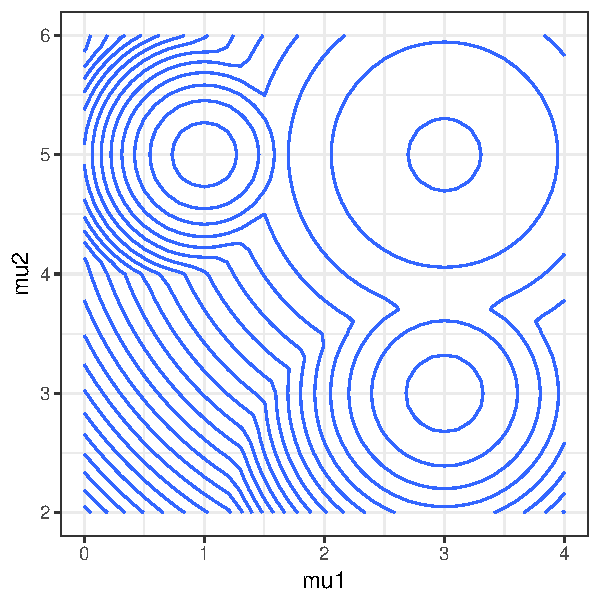
\includegraphics[width=1\textwidth]{fmm_mu_contour.pdf}
    \caption{Posterior density of the component means.}
    \end{subfigure}
    \end{center}
    \centering
   \begin{subfigure}[b]{0.32\textwidth}
    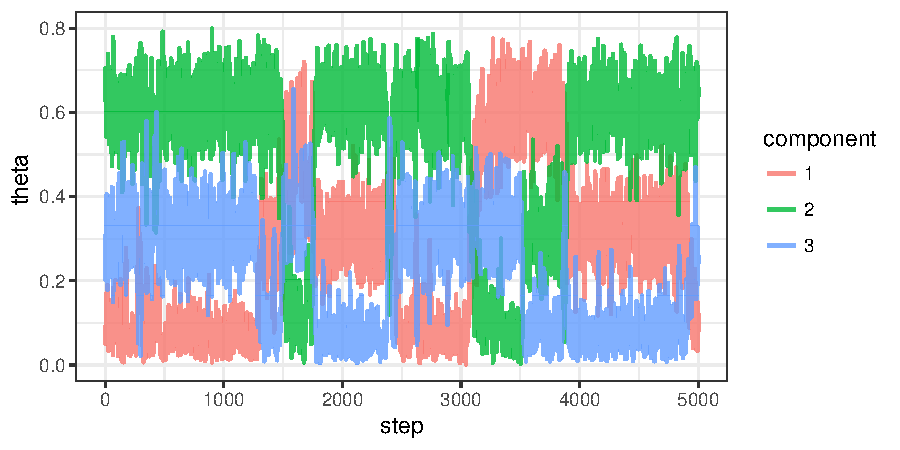
\includegraphics[width=1\textwidth]{fmm_w_gibbs.pdf}
    \caption{Gibbs sampling under canonical Dirichlet}
    \end{subfigure}
       \begin{subfigure}[b]{0.32\textwidth}
  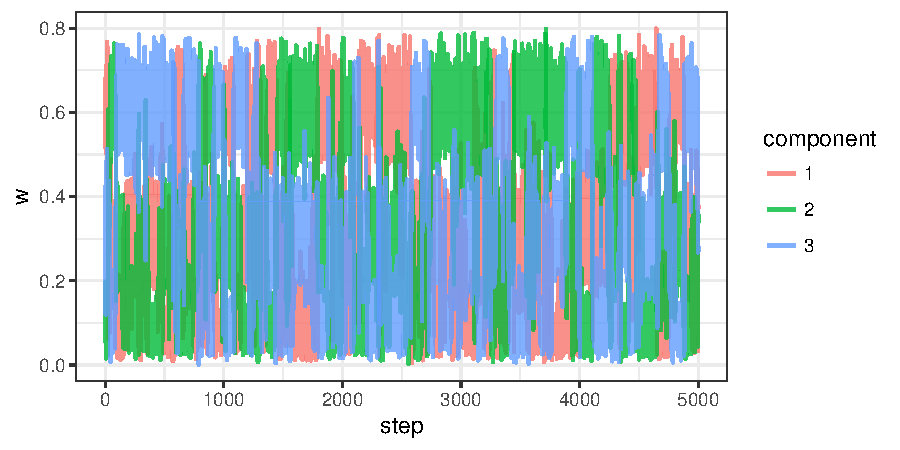
\includegraphics[width=1\textwidth]{fmm_w_hmc_unordered.pdf}
    \caption{HMC sampling under canonical Dirichlet, using extrinsic prior}
      \end{subfigure}
       \begin{subfigure}[b]{0.32\textwidth}
 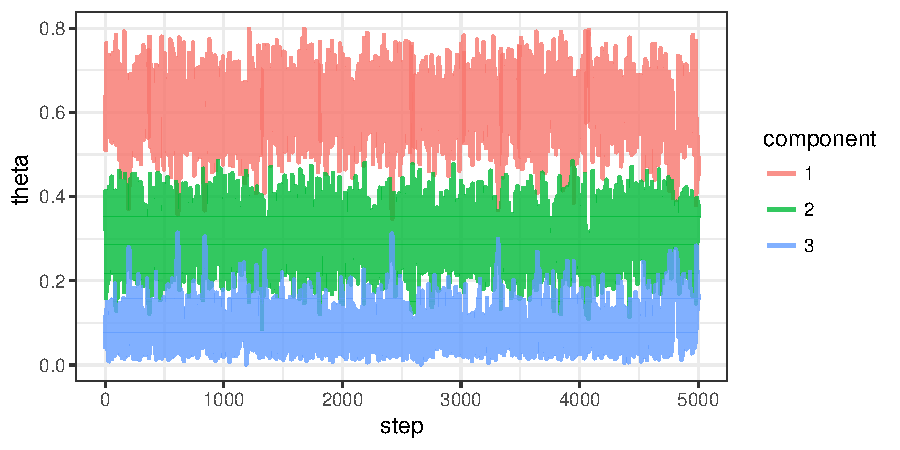
\includegraphics[width=1\textwidth]{fmm_w_hmc.pdf}
     \caption{HMC sampling under ordered Dirichlet, using extrinsic prior}
     \end{subfigure}
\caption{Contour of the posterior density of component means and traceplot of the posterior sample for the component weights, in a 3-component normal mixture model. Panel (a) shows that there is significant overlap among component means, creating label-switching issues in both Gibbs sampling (b) and HMC sampling using canonical prior (c). The ordered Dirichlet prior, estimated under extrinsic prior and correcting projection, significantly reducing label-switching (d).}
\label{dirichlet}
\end{figure}


{\bf Example 2: Orthonormal Gaussian Processes in Functional Principle Component Analysis}

\leo{There are some issues with this model. Skip it for now.}

We now consider functional principle component analysis. Letting $x_i$ be the input for $i=1,\ldots,n$ in functions $f_j(x_i)$ for $j=1,\ldots,p$. We observe functional data $y_{i,j}$ as noisy realizations of $f_j(x_i)$. Commonly, $p$ is very large and it is useful to view the functions as linear combination of $d$ functional factors $g_k$.

\begin{equation*}
\begin{aligned}
y_{ij} & = f_j(x_i) + \epsilon_{ij},\\
 f_j(x_i) & = \sum_{k=1}^{d} \eta_{jk} g_k(x_i),\\
 \left [ g_k(x_1) , \ldots , g_k(x_n) \right] &\sim \No (0, \Sigma_k)\\
\Sigma_{k,(i,i')} &= \phi_k\exp( - \frac{||x_i-x_{i'}||^2}{2\rho_k^2})
\end{aligned}
\end{equation*}
for $k=1,\ldots d$ with $d<p$, and $\epsilon_{ij}\sim \No(0,\sigma^2)$ is the random measurement error; $\Sigma_{k,(i,i')}$ is the $(i,i')$th element in matrix $\Sigma_k$. Using matrix notation $G=[g_1, \ldots, g_d]$ and $\eta= [\eta_{.1},\ldots,\eta_{.d}]$, the $n\times p$ function matrix $[f_j(x_i)]_{ij}$ can be written as $G \eta'$. We utilize a squared exponential Gaussian process to model each latent factor $g_k$.

We first assign a shrinkage prior on loadings $\eta_{jk}\sim \No(0,\tau_k)$, $\tau_k \sim IG(aq^{3(k-1)},q^{2(k-1)})$  with $q>1$. This prior ensures the shrinkage grows stronger as $k$ increases \citep{bhattacharya2011sparse}, avoiding arbitrary specification of $d$ and exchangability in permuting $k$. However, $G$ and $\eta$ are still not identifiable. Any orthonormal matrix $P$ that $P'P = I_d$ can produce another set of factors $G^*= GP'$ and loadings $\eta^* = P\eta$. Since this projection $P$ is associated with rotation, scaling or column-wise sign change, we apply the following constraint on $G$:

\begin{equation*}
\begin{aligned}
 \sum_{i=1}^n g_k(x_i) g_{k'}(x_i) &= \left\{ \begin{array}{cc}1 \text{ if } k=k' \\ 0 \text{ if } k \neq k'\end{array}\right. \\
 g_k(x_1) \ge 0
\end{aligned}
\end{equation*}
for $k=1,\ldots d$. The orthonormailty restricts rotation and scaling and $g_k(x_1)\ge 0$ restricts column-wise sign change. 

As the result, these constraints create a Gaussian process prior on a Stiefel manifold $\mc V(N,d)$. To our best knowledge, this is the first application of Gaussian process in this manifold. We approximate these constraints with extrinsic prior:

 \begin{equation*}
\begin{aligned}
\pi_{\mc K}(G) \propto   \prod_{k=1}^{d} K_{1}{\left((-g_k(x_1) )_+\right)} \cdot \prod_{k'=1}^{d}\prod_{k=1}^{k'} K_2 ( |\sum_{i=1}^n g_k(x_i) g_{k'}(x_i) - \delta_{k,k'}|)
\end{aligned}
\end{equation*}
where $K_{k}(x)=\exp(- \lambda_k x^2) \1_{x<4/\sqrt{2\lambda_k}}$ for  $k=1,2$. We use $\lambda_1 = 10^6$ to strongly enforce the sign of $g_k(x_1)$ to be positive, while $\lambda_2 = 10^3$ to allow efficient mixing in embedding Stiefel manifold in $\mathbb{R}^{N\times d}$. To compare with unconstrained Gaussian processes for $g_k$'s, we also test with $\lambda_1=0$ and $\lambda_2=0$.

We generate $n=50$ inputs $x_i\sim \text{U}(0,1)$ from uniform $(0,1)$ and three smooth functions $g^*_1(x)= \sin(16 x)/x$, $g^*_2(x)= \sin(25 x)\cdot x$ and $g^*_3(x)= \cos(20 x)/x$. The functions are combined via $f_j(x_i)=\sum_{i=1}^3 \eta^*_{jk} g^*_k(x_i)$ with $\eta^*_{jk}\stackrel{iid}{\sim} \No(0,1)$ for $j=1,\ldots,20$ and $i=1,\ldots,n$. We add random noise to create a $50\times 20$ data points $y_{ij} \sim \No(f_j(x_i),0.1^2)$, and randomly remove $20\%$ of data to mimic the unbalanced data in real world. We set $a=q=2$ in the shrinkage prior for all $\eta_{jk}$'s, uniform prior $\text{U}(0,20)$ for all $\rho_k$'s, $\phi_k$'s and $\sigma^2$.

{\bf Example 3: Orthonormal Tucker Factorization in Multiple Network Analysis}


\section{Discussion}



\bibliography{reference}
\bibliographystyle{chicago}

\end{document}



We now illustrate a curve fitting problem where the shape of curve is convex. Convexity is common in real life such as a trajectory of projectile or accelerated decreasing of organ functions in disase monitinoring. Consider a cubic spline function $f(t)$ for data $y_t$ with $t\in [0,1]$


\begin{equation*}
\begin{aligned}
y_t & = f(t) + \epsilon_t,\\
f(t) & = \beta_0 + \beta_1 t + \beta_2 t^2+ \beta_3 t^3+ \sum_{j=1}^J b_j (t- \tau_j)^3_+,\\
\end{aligned}
\end{equation*}
where $\epsilon_t \sim \No(0, \sigma^2)$ and $\tau_j$'s are pre-specified knots in $(0,1)$. To induce the convexity, it suffices to have the second derivative:

\begin{equation*}
\begin{aligned}
f''(t) & =  2\beta_2 + 6\beta_3 t+ \sum_{j=1}^J 6b_j (t- \tau_j)_+ \ge 0.\\
\end{aligned}
\end{equation*}

Given data $y_t$ at observed time $t=t_1,\ldots, t_n$, the posterior estimation of $\beta_.$ and $b_.$ is estimated under $n$ linear inequality constraints.

